\section{Методология и Инструментарий}

Для решения задачи автоматизации метаморфизма кода Go с использованием больших языковых моделей была разработана и реализована специализированная методология, воплощенная в программном инструментарии. Основой инструментария является модульная архитектура, реализованная на языке Go, что обеспечивает гибкость, производительность и удобство разработки. Проект структурирован с разделением на пользовательский интерфейс командной строки и внутреннюю логику преобразования кода.

Центральным компонентом системы является пакет \texttt{internal/rewriter}, инкапсулирующий всю логику, связанную с метаморфическими преобразованиями. Ключевая особенность данного модуля заключается в том, что он выступает в роли абстрактного интерфейса к внешним LLM, не реализуя самостоятельно алгоритмы обфускации. Его задача — получить фрагмент исходного Go-кода, сформулировать соответствующий запрос к выбранной модели нейронной сети и обработать ее ответ. Пакет поддерживает работу с различными API нейронных сетей, выбор конкретного API осуществляется через перечисление \texttt{APIType} (например, поддерживаются варианты для Gemini и OpenRouter). Фабричная функция \texttt{NewLLMRewriterWithAPI} отвечает за создание экземпляра переписчика, сконфигурированного для работы с указанным API. Основные методы переписчика включают \texttt{RewriteFile}, который читает содержимое входного файла и инициирует процесс его переписывания через LLM, и \texttt{SaveRewrittenFile}, сохраняющий полученный результат.

Взаимодействие с LLM является ядром процесса метаморфизма в данной архитектуре. Модуль переписывания формирует запрос, включающий исходный фрагмент кода и текстовый промпт. Именно промпт инструктирует нейронную сеть выполнить преобразование, соответствующее одной из целевых техник метаморфизма: вставки "мертвого"\, кода или модификации потока управления. Качество генерации метаморфического варианта напрямую зависит от точности и ясности этого промпта, а также от способности конкретной LLM интерпретировать инструкции и генерировать семантически эквивалентный, но структурно измененный Go-код. Предполагается, что модели, обученные на больших кодовых корпусах \cite{Chen21Evaluating}, обладают необходимыми возможностями для выполнения таких преобразований.

\begin{figure*}[h!] % Начать окружение figure. htbp - параметры размещения
    \centering % Центрировать содержимое фигуры

    % --- Первая строка (2 изображения) ---
    \begin{subfigure}[b]{0.5\textwidth} % Ширина чуть меньше половины для двух фото
        \centering
        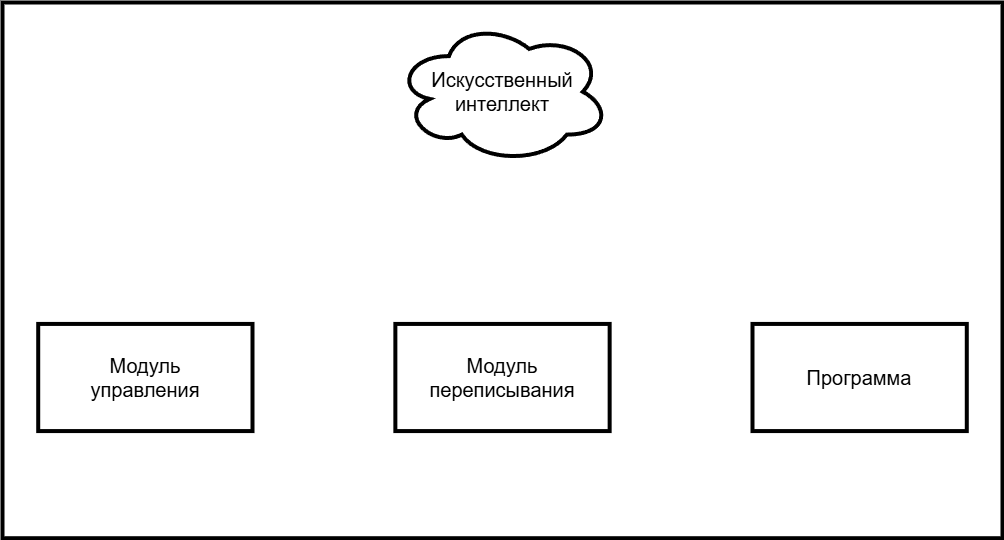
\includegraphics[width=\textwidth]{images/METAMORPHLLM0.png} % Укажите путь к фото 1
        \caption{Этап 1}
        \label{fig:photo_221_1}
    \end{subfigure}% <-- Важный % для удаления пробела
    \hfill % Добавить растяжимое пространство между изображениями
    \begin{subfigure}[b]{0.5\textwidth}
        \centering
        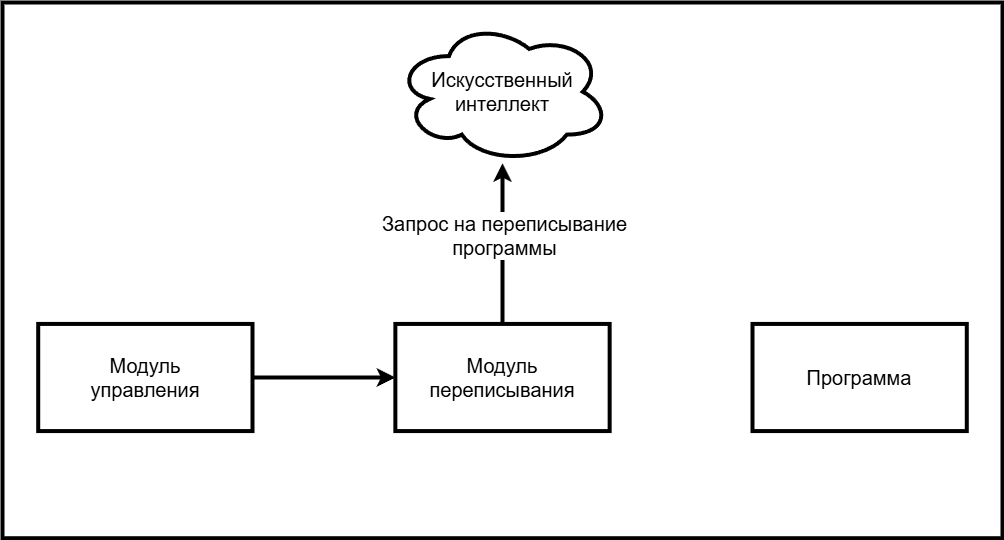
\includegraphics[width=\textwidth]{images/METAMORPHLLM1.png} % Укажите путь к фото 2
        \caption{Этап 2}
        \label{fig:photo_221_2}
    \end{subfigure}

    \vspace{\baselineskip} % Добавить вертикальный отступ между строками

    % --- Вторая строка (2 изображения) ---
    \begin{subfigure}[b]{0.5\textwidth}
        \centering
        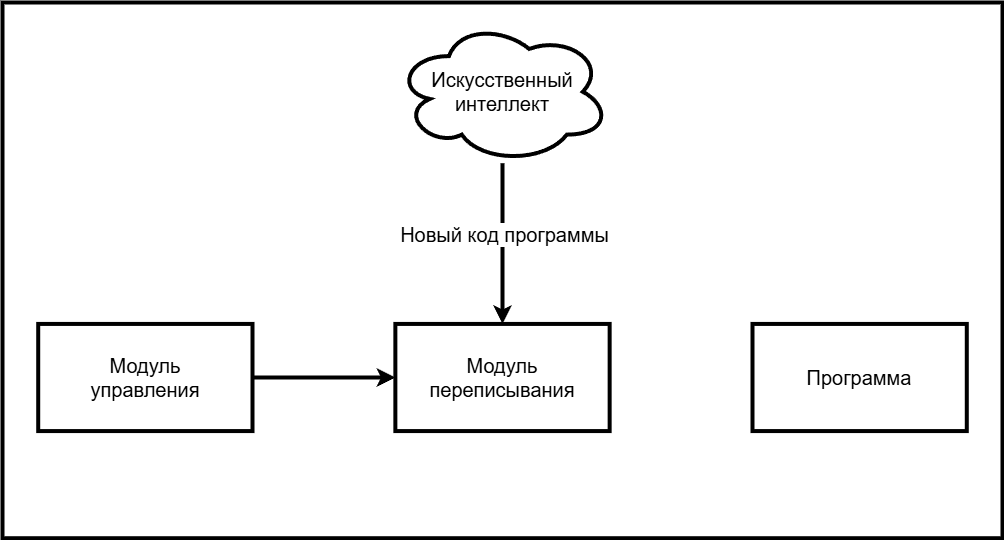
\includegraphics[width=\textwidth]{images/METAMORPHLLM2.png} % Укажите путь к фото 3
        \caption{Этап 3}
        \label{fig:photo_221_3}
    \end{subfigure}% <-- Важный %
    \hfill % Растянуть пространство
    \begin{subfigure}[b]{0.5\textwidth}
        \centering
        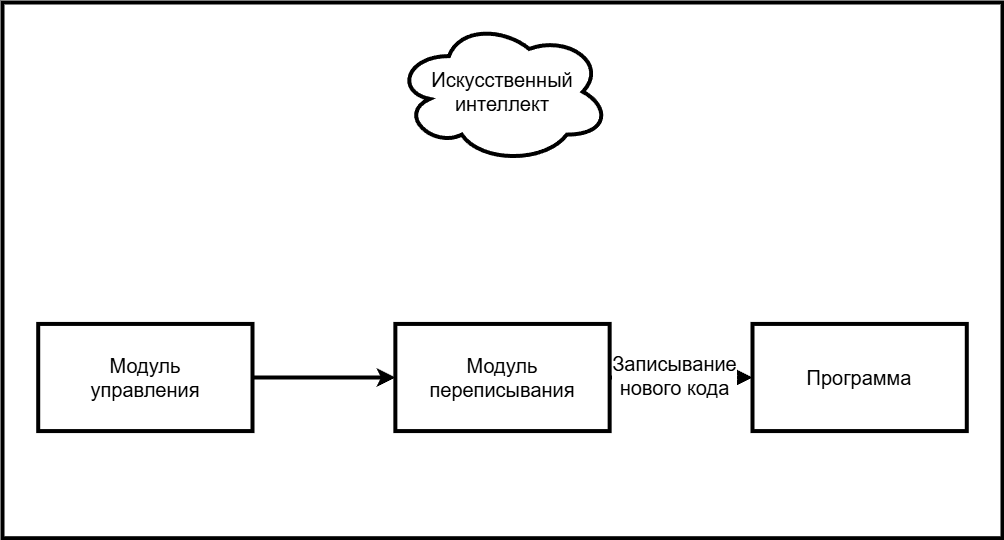
\includegraphics[width=\textwidth]{images/METAMORPHLLM3.png} % Укажите путь к фото 4
        \caption{Этап 4}
        \label{fig:photo_221_4}
    \end{subfigure}

    \vspace{\baselineskip} % Добавить вертикальный отступ между строками

    % --- Третья строка (1 изображение) ---
    % Так как \centering уже есть для всей figure, subfigure будет по центру
    \begin{subfigure}[b]{0.5\textwidth} % Можно сделать шире, если нужно, например 0.5\textwidth
        \centering
        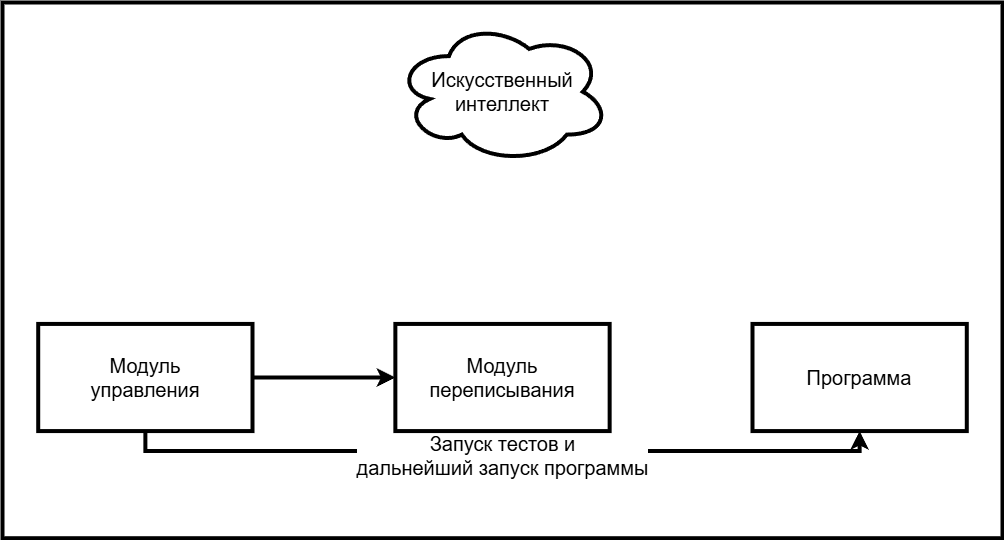
\includegraphics[width=\textwidth]{images/METAMORPHLLM5.png} % Укажите путь к фото 5
        \caption{Этап 5}
        \label{fig:photo_221_5}
    \end{subfigure}

    % --- Общая подпись ко всей группе ---
    \caption{Общая схема работы инструментария.}
    \label{fig:my_five_photos_221} % Метка для ссылки на всю группу

\end{figure*} % Закончить окружение figure

Пользовательский интерфейс реализован в виде CLI-приложения. Этот компонент отвечает за парсинг аргументов командной строки, таких как путь к входному файлу, путь для сохранения результата и выбор используемого API нейронной сети. После валидации входных данных и выбора API, CLI создает экземпляр переписчика из пакета \texttt{internal/rewriter} и вызывает его методы для выполнения основной задачи.

Типичный сценарий работы инструментария выглядит следующим образом: пользователь запускает CLI, указывая исходный файл, желаемый выходной файл и используемый API LLM. Приложение парсит аргументы, создает соответствующий объект переписчика. Переписчик читает исходный файл, формирует и отправляет запрос, включая код и промп, к API выбранной нейронной сети. Получив ответ с модифицированным кодом, переписчик сохраняет результат в указанный выходной файл.

После записи модифицированного кода в файл, проводится замер метрик с выводом результатов в командную строку

Такая архитектура обладает рядом преимуществ. Четкое разделение логики CLI и ядра переписывания упрощает поддержку и тестирование. Добавление поддержки новых LLM API или даже новых техник метаморфизма путем изменения логики формирования промптов требует модификации только внутреннего пакета \texttt{internal/rewriter}, не затрагивая пользовательский интерфейс. Это обеспечивает хорошую расширяемость инструментария.

Оценка качества сгенерированного метаморфического кода проводится на отдельном этапе с использованием метрик функциональной эквивалентности ($FE$), изменения количества строк кода ($LOC_{fin}$), цикломатической сложности ($CC_{fin}$) \cite{McCabe76Complexity} и когнитивной сложности ($CogC_{fin}$) \cite{SonarSourceCogC}, что позволяет количественно измерить как корректность преобразований, так и достигнутый уровень обфускации.